\documentclass[a4paper]{report}

\usepackage[utf8]{inputenc}
\usepackage[ngerman]{babel}

\usepackage{graphicx}
\usepackage{color}



\title{Abschlussbericht des Systemtechnikprojektes im Studiengang Systems Engineering}
\author{
  Erik Rother\\
  \and
  Lisa Schade\\
  \and
  Kira Löper\\
}
\date{28.09.2018}

\begin{document}

\maketitle

\tableofcontents

\chapter{Einleitung}
In der Mikrostrukturierung optischer Bauteile werden Diamantwerkzeuge mit sehr kleinen Schneidenradien eingesetzt. Die Detektion des Werkzeugkontaktes kann nur durch eine Kamera realisiert werden. Die genau Positionierung der Kamera und die Veränderung der Position sind sehr zeitaufwändig. Während unseres Projektes haben wir uns mit diesem Problem beschäftigt und als Lösung eine elektrisch gesteuerte Kameraführung mit automatischer Werkzeugdetektion entwickelt. In diesem Bericht möchten wir den Prozess der Entwicklung und unsere Resultate beschreiben. 

\chapter{Stand der Technik}
Die automatische Werkzeug-Kontakt-Detektion dient zur Unterstützung der Werkzeug-Positionierung bei mehreren Prozessen. Im Folgenden werden zwei Prozesse vorgestellt, die durch die automatische Werkzeug-Kontakt-Detektion zeiteffizienter gestaltet werden können. \\ \\
Zur Einordnung dieser Prozesse dient Abbildung 2.1. Es sind einige Verfahren zur Herstellung strukturierter optischer Komponenten nach ihrer Komplexität sortiert aufgeführt. Des Weiteren kann man der Abbildung ihre Dimensionen und Anwendungen entnehmen. \\ \\ 
\begin{figure}[htbp]
\centering 
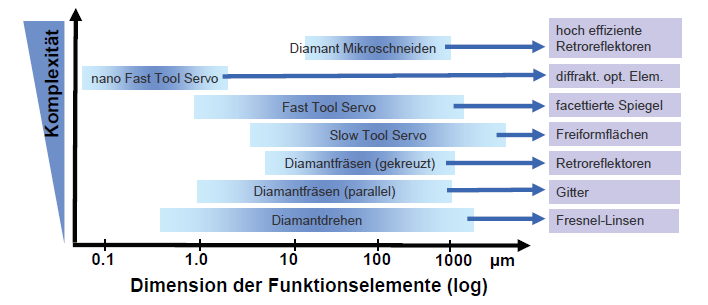
\includegraphics[width=0.8\textwidth]{Fertigungsverfahren.PNG}
\caption{Werkzeug zum Mikroschneiden}
\label{fig:Bild1}
\end{figure}
\break

\section{Diamant-Mikroschneiden}
Das Diamant-Mikroschneiden dient zur Herstellung von prismatischen Mikrokavitäten mit scharfkantig aufeinandertreffenden Facettenflächen, wie sie zum Beispiel bei retroreflektierenden Strukturen erforderlich sind. Um retroreflektierende Strukturen zu fertigen werden aus glatten Oberflächen gezielt bestimmte Bereiche entfernt und die reflektierende Struktur bleibt stehen. Das Diamant-Mikroschneiden unterschiedet sich durch seine Werkzeuge und Kinematik grundlegend von anderen Fertigungsverfahren. \\ \\
Abbildung 2.2 zeigt das Diamant-Werkzeug, welches sich dadurch auszeichnet, dass Span-und Freifläche gegeneinander vertauscht wurden. \\ \\
\begin{figure}[htbp]
\centering 
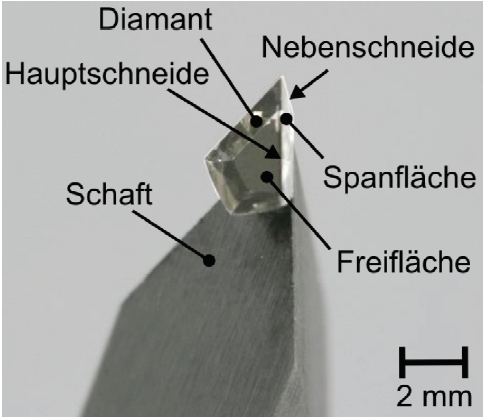
\includegraphics[width=0.3\textwidth]{Werkzeug.PNG}
\caption{Werkzeug zum Mikroschneiden}
\label{fig:Bild2}
\end{figure}
\break
Abbildung 2.3 zeigt die Kinematik des Mikroschneidens. Das Werkzeug schneidet zunächst in X,Y,-Z Richtung in das Werkstück und wird anschließend in -X,Y,Z Richtung zurückgeführt. Anschließend wird das Werkstück rotiert und der Schnittvorgang wiederholt sich. Durch diesen Vorgang können drei- bis sieben-seitige Kavitäten erstellt werden. \\ \\
Außerdem ist die Herstellung von kubischen Retroreflektoren aus dreieckigen Einzelstrukturen abgebildet. \\ \\
\begin{figure}[htbp]
\centering 
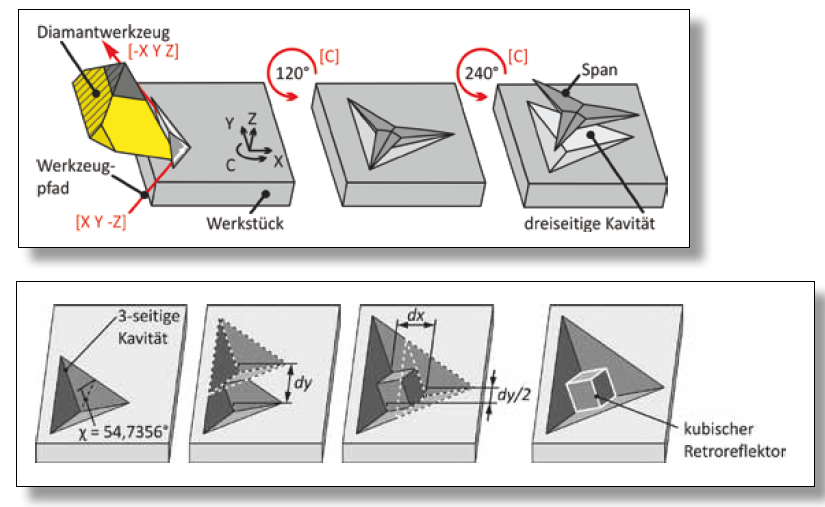
\includegraphics[width=0.8\textwidth]{Mikroschneiden_Kinematik.PNG}
\caption{Kinematik des Mikroschneidens}
\label{fig:Bild3}
\end{figure}
\break
\\ \\
Besonders wichtig beim Mikroschneiden ist die richtige Justierung des Werkzeuges innerhalb der Maschine. Hier muss eine Genauigkeit von unter einem Mikrometer in allen Raumrichtungen erreicht werden. Sonst würden sich die einzelnen Spiegelflächen der Strukturen nicht präzise treffen und die gewünschte optische Funktion ließe sich nicht erreichen.




\section{nano Fast Tool Servos (nFTS)}
Das Verfahren nano Fast Tool Servos dient zur Herstellung diffraktiver optischer Komponenten, welche ihre Anwendung beispielsweise in der Sicherheitstechnik finden. Dieses Verfahren arbeitet mit einer speziellen piezoelektrischen Keramik, welche sich durch eine hohe Linearität und geringe Hysterese auszeichnet. Darauf befindet sich eine Montageplatte für das Diamantwerkzeug. 

\chapter{Konzeptentwicklung}

Nachdem wir uns mit der Problematik der Kamerapositionierung zur Werkzeugkontakt-Detektion beschäftigt haben, wurden erste Lösungsansätze erarbeitet. Die grundlegende Fragestellung befasste sich damit, welche Art der Kameraführung am besten für das gegebene Problem geeignet ist. Bei der Beurteilung galt es zu überprüfen, ob die Grundstrukturen die gegebenen Anforderungen erfüllen und dabei gleichzeitig wirtschaftlich sind. In der nachfolgenden Tabelle sind vier Grundstrukturen der Kameraführung mit ihren Vor- und Nachteilen aufgelistet. \\ \\

\begin{tabular}{lll}
 
Grundstruktur der Kameraführung & pro & contra \\
 \hline
 \hline
Raumportal & schnell & groß \\
 & präzise & schwer \\
& größere Lasten möglich &\\
  \hline
Gimbal & leicht & Änderung der Führung notwendig \\
 & schnell & \\
& preiswert & \\
 \hline
Parallelkinematik & sehr präzise & sehr teuer\\
&  enorm flexibel & zweite Führung notwendig \\
  \hline
Tragarm & sehr günstig  & Hebelwirkung vermindert Stabilität\\

\end{tabular}
\\ \\
\\ \\
Das Raumportal bietet zwar viele Vorteile um eine Kamera genau und schnell im Raum auszurichten, ist jedoch für unsere Anforderungen nicht optimal, da es sehr viel Platz einnimmt. Es ist wichtig, dass unsere Kameraführung die Arbeit der Maschine nicht beeinträchtigt, sodass wir uns gegen das Raumportal entschieden haben. \\ \\
 Die Parallelkinematik bietet eine sehr präzise Ausrichtung der Position und kann eine Beweglichkeit in allen sechs Freiheitsgraden ermöglichen zum Beispiel in Form eines Hexapods. Die Bewegungen sind jedoch auch sehr klein, sodass wahrscheinlich eine zweite Führung notwendig wäre, um die Position der Kamera zunächst grob einzustellen. Die Parallelkinematik ist auch sehr teuer, sodass wir diese Lösung nicht als wirtschaftlich ansehen. \\ \\
Im Gegensatz dazu wäre ein Tragarm eine sehr preiswerte Lösung. Jedoch könnte es zu Problemen in der Stabilität kommen, wenn die Hebelwirkung an dem Tragarm zu groß wird. Außerdem sind preiswerte Tragarme manuell einzustellen, was nicht den Anforderungen entspricht. \\ \\
Der Gimbal erschien uns als eine gute Grundlage für das Kamera-Positionierungssystem, da er leicht, schnell und preiswert ist. Der Gimbal enthält drei bürstenlose Motoren mit denen sehr kleine Winkeländerungen möglich sind. Den mechanischen Teil der Führung würden wir auf unsere Anforderungen anpassen. Wir haben uns also für diese Variante der Kameraführung entschieden. \\ \\

TO DO ÜBERARBEITUNG

\chapter{Aufbau des Gesamtsystems}
TO DO BILD \\ \\
Folgende Geräte und Bauteile wurden verwendet
\begin{itemize} 
\item Kamera: Guppy F - 146
\item Objektiv: Macro-CCD Lens 4x
\item Laptop mit FireWire-Schnittstelle
\item Raspberry Pi 2 Model B 
\item Bildschirm, Tastatur, Maus (einschließlich Kabel zum Anschließen an den Raspberry Pi)
\item  Crossover-Kabel
\item  TO DO Motoren: BGM4108-130, ESC: STorM32BGC, F35A 3-6S BLHeli\_32...
\item Schaltung: Mikrocontroller: (L293D), Widerstände (1k Ohm), Brücken
\end{itemize}
Die Position der Kamera ist durch ein Gestell mit drei Motoren variabel, wodurch ihr Winkel so eingestellt werden kann, dass sich Werkzeug und Werkstück optimal im Bildausschnitt befinden. Das Gestell kann sowohl an der Werkzeughalterung, als auch über der Werkstückaufnahme montiert werden. Im Rahmen unseres Projektes konnten wir die Montage TO DO realisieren.
Die Kamera ist über eine FireWire-Schnittstelle mit dem Laptop verbunden. Der Laptop speichert das Bildmaterial und stellt es per Ordnerfreigabe dem Raspberry Pi zur Verfügung. Bildschirm, Maus und Tastatur sind an dem Raspberry Pi angeschlossen, sodass der Benutzer mit Hilfe einer graphischen Oberfläche gewünschte Aktionen auswählen kann. Außerdem verfügt der Raspberry Pi über einen Algorithmus, der zusammenhängende Bereiche mit bestimmten Farbwerten erkennt, wodurch die Kamera automatisch dem Werkzeug folgen kann. (TO DO kann sie das?)

\chapter{Datenübertragung}
Die automatische Positionierung der Kamera setzt voraus, dass die Daten über den aktuellen Bildausschnitt bekannt sind. Die Kamera verfügt über eine FireWire-Schnittstelle. FireWire-Schnittstellen besitzen eine hohe Datendurchsatzrate, wodurch ein besonders schnelles Arbeiten möglich ist. FireWire 400 überträgt Datenströme und ist USB 2.0 daher besonders bei der Übertragung von kontinuierlichen Signalen zum Beispiel im Videobereich überlegen. Jedoch hat sich diese Schnittstelle auf dem Markt nicht durchgesetzt, weshalb viele aktuelle Geräte diese Schnittstelle gar nicht besitzen. USB bietet seit USB 3.0 eine so deutlich überlegene Übertragungsgeschwindigkeit, dass auch im Videobereich größere Datenraten übertragen werden können. \\ \\
Zur Verfügung steht uns ein Laptop der Firma Toschiba mit dem Betriebssystem Windows XP. Dieser bietet einen FireWire-Anschluss, sodass wir die Kamera anschließen können. Das Bildmaterial der Kamera wird mit einer Software von MatLab auf dem Laptop angezeigt und abgespeichert. Da dieser Laptop jedoch sehr langsam arbeitet, wird die weitere Verarbeitung der Bilddaten auf einen Raspberry Pi 2 Model B ausgelagert. \\ \\
Zur Übertragung der Bilddaten nutzen wir das Prinzip der Ordnerfreigabe. Das Betriebssystem Windows XP unterstützt Netzwerkfreigaben von sich aus, während der Raspberry Pi ein zusätzliches Programm für diese Funktion benötigt. Zum Einbinden der Windows-Freigabe nutzen wir das virtuelle Dateisystem \glqq cifs-vfs\grqq. Dazu wird das Paket \glqq cifs-utils\grqq auf dem Raspberry Pi installiert. Um den freigegebenen Ordner in das Dateisystem einzubinden nutzen wir den Befehl \glqq mount\grqq, wobei auch der Typ \glqq cifs\grqq und Angaben über den Ort des freigegebenen Ordners, sowie des Zielordners notwendig sind. Damit man den Ordner nicht bei jedem Neustart des Raspberry Pi's neu einbinden muss, hinterlegen wir alle Informationen für das Einbinden in der Konfigurations-Datei \glqq /etc/fstab\grqq. Nun müssen nur noch mit einem Befehl alle Dateisysteme, die in \glqq /etc/fstab\grqq vermerkt sind, einbinden. Dieser Befehl wird bei öffnen der graphischen Oberfläche unseres Programms automatisch ausgeführt. \\ \\
Für die Verbindung zwischen Laptop und Raspberry Pi gibt es mehrere Möglichkeiten. Wir haben uns mit den zwei Möglichkeiten beschäftigt. \\ \\
 Die erste Möglichkeit ist die Verbindung über das Netzwerk im LFM. Beide Geräte sind durch ein Ethernet-Kabel mit dem Netzwerk verbunden. Ein Vorteil ist, dass die Geräte auch so Zugang zum Internet haben. Der Laptop benötigt den Zugang zum Internet um die notwendigen Lizenzen für MatLab laden zu können. Der freigegebene Ordner kann nun in dem Netzwerk durch Angabe der IP-Adresse des Laptops im Netzwerk und Angabe des Freigabenamens gefunden werden. Dieser Ordner ist nun mit jedem Gerät in dem Netzwerk auffindbar, jedoch ist der Zugriff durch das Passwort des Benutzerkontos von dem Laptop geschützt. \\ \\
Die zweite Möglichkeit ist eine direkte Verbindung durch ein Crossover-Kabel. Diese Verbindung ist sicherer und die Daten können schneller übertragen werden. Jedoch ergibt sich das Problem, dass das Crossover-Kabel den gleichen Anschluss verwendet, wie das Ethernet-Kabel. So kann der Laptop nicht gleichzeitig mit dem Raspberry Pi verbunden sein und Zugang zum Internet haben. Den Internetzugang braucht er allerdings, um die MatLab-Lizenzen zu laden. So müsste zuerst das Ethernetkabel angeschlossen werde, sodass die Lizenzen laden können. Danach müsste man das Kabel entfernen und das Crossoverkabel anschließen, um die Verbindung zum Raspberry Pi herzustellen. Dies wäre nicht besonders anwenderfreundlich. Jedoch konnte diese Möglichkeit optimiert werden, indem durch einen Adapter ein zweiter Netzwerkanschluss an dem Laptop angebracht wurde. Dies ermöglicht Internetzugang mit einem Ethernet-Kabel und mit dem Crossoverkabel diei Verbindung zum Raspberry Pi. Die IP-Adressen werden bei dieser Variante statisch gesetzt. So hat der Laptop die IP-Adresse \glqq 192.168.1.1\grqq und der Raspberry Pi die IP-Adresse  \glqq 192.168.1.2\grqq erhalten. Beiden wurde die gleiche Subnetzmaske  \glqq 255.255.0.0\grqq \\ übergeben. So kann der Ordner wieder durch die IP-Adresse des Laptops und den Freigabenamen gefunden und in das Dateisystem von dem Raspberry Pi einghängt werden. Mit dieser Variante wird nur ein LAN-Anschluss am Einsatzort des Systems benötigt und eine schnelle und sichere Datenübertragung ermöglicht, sodass wir uns für diese Variante entschieden haben. \\ \\
Durch die Arbeit mit mehreren Raspberry Pis benötigten wir die Einstellung, dass der Ordner für alle Benutzer freigegeben ist. Da der Laptop bei unserer Variante nun mit dem gesamten Netzwerk des Instituts verbunden ist, könnte man als eine zusätzliche Sicherheit (neben dem benötigten Passwort) die Ordnerfreigabe auf einen Benutzer beschränken. Dies müsste noch einmal durch einen Administrator des Laptops geschehen. 

\chapter{Hardwareentwicklung}
\section{Aufbau der Schaltung}
TO DO
\section{Steuerung der Motoren}
TO DO
\section{Konstruktion des Gestells}
TO DO

\chapter{Algorithmus zur Werkzeugerkennung}

Um die Werkzeugposition im aktuell ausgewählten Bild definieren zu können, haben wir uns überlegt, dies anhand von Pixelfarben zu realisieren. Denn man kann davon ausgehen, dass das Werkzeug in dem aufgenommen Bild größtenteils die gleiche Farbe hat oder nur kleine Farbabweichungen aufweist. Die Abweichungen können im Algorithmus kompensiert werden, je nach gegebenen Bedarf. \\  
Das von der Kamera aufgenommene Bild repräsentiert in Wirklichkeit nur einen ganz kleinen Ausschnitt, der keine weiteren größeren Objekte mit genau dieser Farbe enthalten dürfte. Aus diesem Grund nehmen wir an, dass das größte Objekt in dem Bild mit der ausgewählten Pixelfarbe dem Werkzeug entsprechen muss.

\section{Funktionsweise}
Um das Werkzeug in dem von der Kamera aufgenommen Bild zu finden, muss eine bestimmte Pixelfarbe ausgewählt werden.  Dem User werden bestimmte Farbe schon in der GUI vorgegeben, die der Werkzeugfarbe entsprechen könnten. Des Weiteren kann er jedoch auch eine Farbe selber auswählen, in dem er diese anhand von RGB-Werten eingibt oder mithilfe von einem Klick in das aktuell ausgewählte Bild die gewünschte Farbe definiert. Nun durchsucht der Algorithmus das komplette Bild nach dieser Farbe. Zuvor kann noch entschieden werden, ob nur nach genau dieser Farbe gesucht werden soll oder man einen gewissen Wertebereich zulassen möchte, den man dann selber angeben kann. Beim Durchsuchen des Bildes wird jede Zeile von links nach rechts durchsucht und es werden sogenannte Segmente gebildet, wenn die übergebene Farbe gefunden wurde. Ein Segment besteht dabei aus einem Start- sowie einem Endpunkt und der dazugehörigen Y-Koordinate. Wenn das Segment die angeklickte Position im Bild enthält, wird noch ein Merker gesetzt um dieses Segment als Werkzeug zu markieren. Im nächsten Schritt werden nun die Segmente, die zusammenhängen, miteinander verbunden. Segmente gehören zusammen wenn sie über- oder untereinander liegen und sich mit mindestens einem Pixel überlappen. Aus diesen zusammenhängenden Segmenten werden dann Bereiche gebildet. Wenn bei einem Segment aus diesem Bereich der Merker gesetzt ist, wird auch für den ganzen Bereich der Merker gesetzt, denn dann ist der ganze Bereich das Werkzeug. Wurde jedoch die Farbe durch eine Eingabe definiert oder eine der vorgegeben Farben ausgewählt, so werden die verschiedenen Bereiche durchlaufen und der mit der größten Anzahl an Pixeln, wird als Werkzeug definiert. Denn es ist davon auszugehen, dass es in dem kleinen Bildausschnitt nicht noch ein weiteres Objekt gibt, welches genau die gleiche Farbe hat.


\chapter{Graphische Oberfläche}
In der GUI werden dem User verschiedene Möglichkeiten geboten, die Motoren einfach ansteuern zu können oder sogar automatisch an eine gewünschte Position verfahren zu lassen.  Des Weiteren ist die graphische Oberfläche dazu da, um Berechnungen, die im Hintergrund ausgeführt werden, zu starten und deren Ergebnisse wiederum an andere Funktionen weiterzuleiten, die die zuvor berechneten Werte als Eingabe benötigen.
Eine weiter wichtige Aufgabe ist das Anzeigen des aktuell aufgenommen Bildes der Kamera, welches das Werkzeug sowie Werkstück enthält. Jedoch besteht nicht nur die Möglichkeit sich das aktuelle Bild anzusehen, man kann sich auch noch zuvor aufgenommen Bilder anschauen, um Einstellungen zu vergleichen oder um doch mit früheren Positionen weiterarbeiten zu können.

\chapter{Bedienungsanleitung}
TO DO (erst wenn finale Version fertig ist)
\begin{itemize} 
\item Einschalten, Kamera einrichten...
\item Bild aufnehmen
\item Bild verschicken (abhängig von Automatisierung)
\item GUI Bilder neu laden Bilder anzeigen
\item verschiedene Methoden zur Motoransteurung
\item zusätzliche Funktionen
\end{itemize}

\chapter{Schlusswort}
TO DO (was funktioniert und Aussicht wie System optimiert werden kann)


\end{document}
